%\documentclass[times]{MGS_class}
%%-----
%%Title und Author angeben
%\title{Software Architecture}
%\author{Florian Krauß, Dino Madach}
%%die Institute weiter unten zu den zugehörigen superscripts angeben
%
%\begin{document}
%
%\twocolumn[{\csname @twocolumnfalse\endcsname
%\begin{center}
%\maketitle
%%\thispagestyle{empty}
%\end{center}
%%\normalsize
%\hspace{15mm}
%
%}]%---

\begin{abstract}
Software architecture is able to grant a lot of benefits in the process of software engineering. Furthermore it supports engineers in avoiding problems occurring during this process. This article will show why software architecture becomes more and more important to the modern world and how it can be presented to any kind of stakeholders. That includes a short description of the most important UML basics and the evaluation of an UML visualisation tool: the Enterprise Architect. Additionally there is an introduction to model driven architecture to present its purposes.
\end{abstract}
\begin{keywords}
Software Architecture, UML, Model Driven Architecture, Enterprise Architect
\end{keywords}

\section{Definition} \label{sec:Introduction}%ein Sternderl (engl. asterisk) \section*{Einleitung} unterdrückt die Nummerierung der Überschriften, dann werden sie in Adobe Reader aber auch nicht im Strukturbaum angezeigt

"Software architecture is about dismantling and assembly with respect to style and aesthetics."
\citep{kruchten1995architectural}
There are a lot of different opinions about what software architecture exactly is. In a historical view the word "architecture" is build from the greek words "arché" (begin, source) and "téchne"  (art, trade). So literally translated it means something like "the first art".  \citep{pfeifer1989etymologisches}

In connection with buildings you could say, the first art, the architecture,  is what has to be done before  constructions can be made. Let take this for software as well. According to \citep{sommerville} in the classic waterfall model there are two phases in software engineering before you start with any implementations. These are analysis and design. "From this perspective it can be handled as a bridge between the initial idea and the beginning of its realization. Specifically software architecture of a software system has to define its components, their interfaces and relations and their externally visible features."\citep{starke2011effektive}

There are two kinds of requirements for software: functional and non-functional. The functional requirements are mostly mandatory and, if you take a closer look at it, often not the reason for project disrupting issues. On the other hand, non-functional requirements like performance, compatibility, extensibility, etc. need far more effort to be achieved. That is also what \citep{starke2011effektive} meant with "architecture creates quality". In conclusion software architecture has three greater purposes:\linebreak

1. It grants a mutual understanding of the problem and provides a common platform for further discussions.

2. If gives an structural overview over the system divided into its components, interfaces and the relations between them. 

3. For later maintenance work or extensions it serves as documentation to the engineers.

You are very lucky if your current project (or maybe the one your looking forward to) is settled "in the open countryside".  But be aware: in software engineering there is an anti-pattern, called "reinventing the wheel". In this case anti-pattern just means: something that often happens in practice, you should really avoid to do. Don't try to reinvent the wheel with your software architecture! If you run across a problem, don't think you are the first engineer that ever had to solve it. There are a whole lot of solutions to well-known and repeatedly arising problems in this field of research. The next section will introduce the most common solutions to you, the so called patterns.


% this is a pagebreak
%\pagebreak
\pagebreak

\section{Architectural Patterns}

"The idea of patterns as a way of presenting, sharing, and reusing knowledge about software systems is now widely used. [...] In this section, I introduce architectural patterns and briefly describe a selection of architectural patterns that are commonly used in different types of systems. For more information about patterns and their use, you should refer to published pattern handbooks" \citep{sommerville}
\subsection{Model View Controller}

\begin{figure}[!hbp]
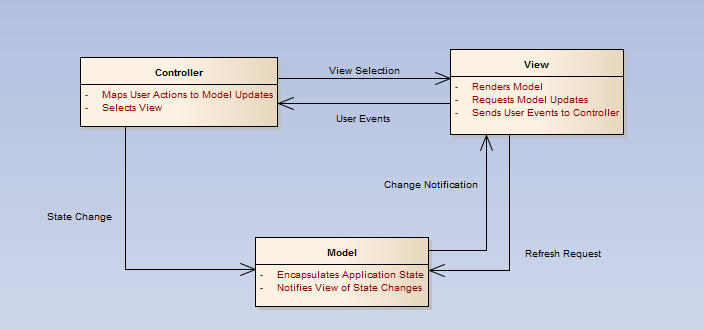
\includegraphics[scale=0.85]{img/pics/mvc.PNG}
\caption{ \protect \cite{sommerville}}
\label{fig:ref_mvc}
\end{figure}


"This pattern is the basis of interaction management in many web-based systems. The stylized pattern description includes the pattern name, a brief description (with an associated graphical model), and an example of the type of system where the pattern is used (again, perhaps with a graphical model). You should also include information about when the pattern should be used and its advantages and disadvantages. A Graphical model of the architecture associated with the MVC pattern is shown in \fref{fig:ref_mvc} which is a conceptual view. A possible run-time architecture when this pattern is used for interaction management in a web-based system would require a browser element in addition." \citep{sommerville}
"Porting an application to another platform shouldn't lead to a revised version of the whole application. Simple changes or extensions and reusability of single components is the goal.
User interfaces changes very often. The same information is to display in different windows in various forms against the complexity of the required frameworks. Different user-groups need different processing.  The difficulty here is to weigh up a consistent view to a model to performance issues, caused by an excessive amount of updates" \citep{starke_rausch}
\vfill
\subsubsection{Advantages}
"Allows the data to change independently of its representation and vice versa. Supports presentation of the same data in different ways with changes made in one representation shown in all of them."\citep{sommerville}
\subsubsection{Disadvantages}
"Can involve additional code and code complexity when the data model and interactions are simple."\citep{sommerville}


\pagebreak

\subsection{Repository}
"[...]the repository pattern \fref{fig:ref_repo} describes how a set of interacting components can share data. The majority of systems that use large amounts of data are organized around a shared database or repository. This model is therefore suited to applications in which data is generated by one component and used by another. Examples of this type of system include command and control systems, management information systems, CAD systems, and interactive development environments for software.
\fref{fig:ref_repo} is an illustration of a situation in which a repository might be used. This diagram shows an IDE that includes different tools to support model-driven development. The repository in this case might be a version-controlled environment [...] that keeps track of changes to software and allows rollback to earlier versions.
\begin{figure}[!hbp]
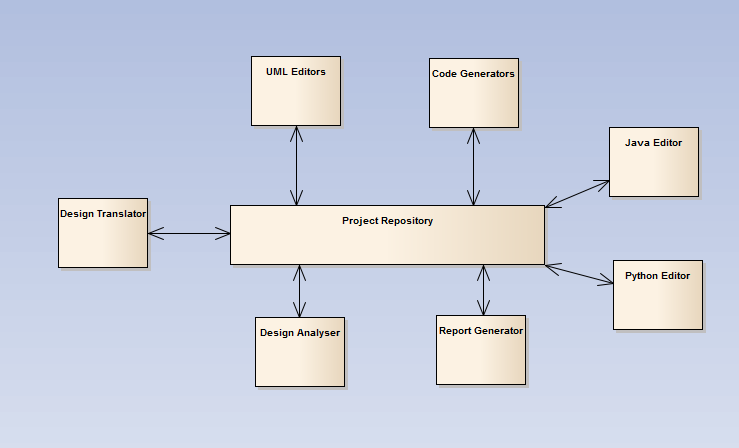
\includegraphics[scale=0.85]{img/pics/Repository.PNG}
\caption{ \protect \cite{sommerville}}
\label{fig:ref_repo}
\end{figure}
Organizing tools around a repository is an efficient way to share large amounts of data. There is no need to transmit data explicitly from one component to another. However, components must operate around an agreed repository data model. Inevitably, this is a compromise between the specific needs of each tool and it may be difficult or impossible to integrate new components if their data models do not fit the agreed schema. In practice, it may be difficult to distribute the repository over a number of machines. Although it is possible to distribute a logically centralized repository, there may be problems with data redundancy and inconsistency.
In the example shown in \fref{fig:ref_repo}, the repository is passive and control is the responsibility of the components using the repository. An alternative approach, which has been derived for AI systems, uses a 'blackboard' model that triggers components when particular data become available. This is appropriate when the form of the repository data is less well structured. Decisions about which tool to activate can only be made when the data has been anylyzed." \citep{sommerville}
\vfill
This pattern is highly recommended when you have large volume of data over a long period of time. In specific, if generated data is able to trigger actions (activate a security tool, start backup, etc.)
\pagebreak
\subsubsection{Advantages}
"Components can be independent - they do not need to know of the existence of other components. Changes made by one component can be propagated to all components. All data can be managed consistently (e.g., backups don at the same time) as it is all in one place."\citep{sommerville}
\subsubsection{Disadvantages}
"The repository is a single point of failure so problems in the repository affect the whole system. May be inefficiencies in organizing all communication through the repository. Distributing the repository across several computers may be difficult."\citep{sommerville}
\subsubsection{Blackboard}
The above mentioned blackboard is defined as the following:
"Several specialised part-systems provide their knowledge to create a possibly incomplete or just approximated solution." \citep{starke_rausch}
\begin{figure}[!hbp]
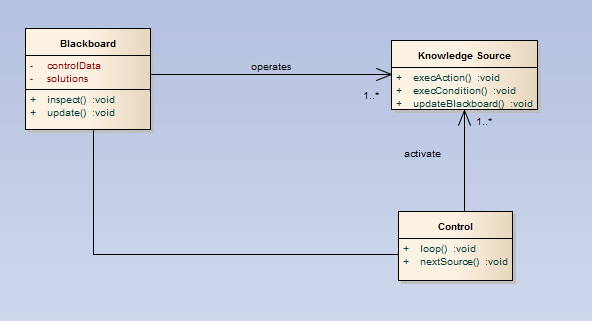
\includegraphics[scale=1.0]{img/pics/blackboard.PNG}
\caption{ \protect \cite{starke_rausch}}
\label{fig:ref_black}
\end{figure}
"Parts of a blackboard are:
- one or multiple independent knowledge sources investigate a problem under specific criterias and send suggested solutions to the blackboard.
- The central blackboard manages the suggested solutions or parts of them sent by the knowledge source.
- The control-component observes the blackboard and controls at needs the execution of the knowledge source." \citep{starke_rausch}\linebreak
The blackboard would be an additional element here. Take the knowledge source as the repository and the control class in \fref{fig:ref_black} as one component. As we already know, components can be reused on other repositories which is a quality criteria for software. Furthermore, the model can be extended as much as you want until it fits your personal needs. 
\pagebreak
\subsection{Client Server}
"The repository pattern is concerned with the static structure of a system and does not show its run-time organization. My next example illustrates a very commonly used run-time organization for distributed systems. The Client-server pattern is described in \fref{fig:ref_cs}.[...]
A system that follows the client-server pattern is organized as a set of services and associated servers, and clients that access and use the services. The major components ofthis model are:
\begin{enumerate}
\item A set of servers that offer services to other components. Examples of servers include print servers that offer printing services, file servers that offer file management services, and a compile server, which offers programming language compilation services.
\item A set of clients that call on the services offered by servers. There will normally be several instances of a client program executing concurrently on different computers.
\item A network that allows the clients to access these services. Most client-server systems are implemented as distributed systems, connected using Internet protocols.
\end{enumerate}
\begin{figure}[!hbp]
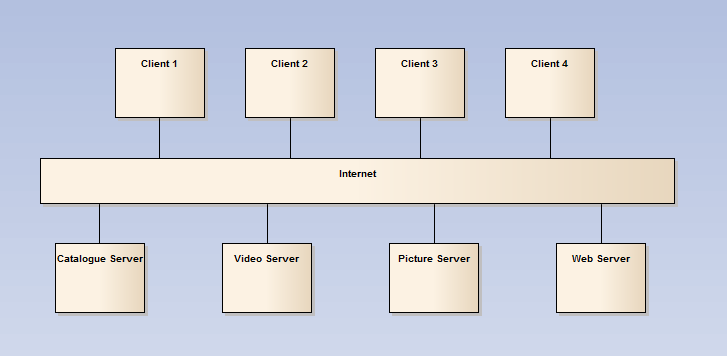
\includegraphics[scale=0.85]{img/pics/Client_Server.PNG}
\caption{ \protect \cite{sommerville}}
\label{fig:ref_cs}
\end{figure}
Client-server architectures are usually thought of as distributed systems architectures but the logical model of independent services running on separate servers can be implemented on a single computer. Again, an important benefit is separation and independence. Services and servers can be changed without affecting other parts of the system.
Clients may have to know the names of the available servers and the services that they provide. However, servers do not need to know the identity of clients or how many clients are accessing their services. Clients access the services provided by a server through remote procedure calls using a request-reply protocol such as the HTTP protocol used in the WWW. Essentially, a client makes a request to a server and waits until it receives a reply.
\fref{fig:ref_cs} is an example of a system that is based on the client-server model. This is a multi-user, web-based system for providing a film and photograph library. In this system, several servers manage and display the different types of media. Video frames need to be transmitted quickly and in synchrony but at relatively low resolution. They bay be compressed in a store, so the video server can handle video compression and decompression in different formats. Still pictures, however, must be maintained at a high resolution, so it is appropriate to maintain them on a separate server." \citep{sommerville} \vfill
\pagebreak
You can find a more simple representation of this model in \citep{starke_rausch} who describes it more general as "service oriented architectures"
\begin{figure}[!hbp]
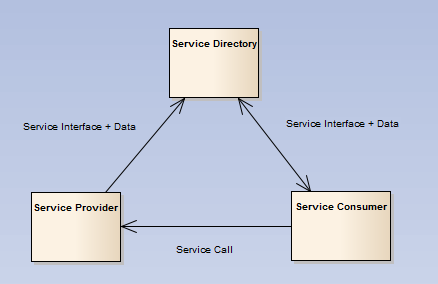
\includegraphics[width=0.9\columnwidth]{img/pics/soa.PNG}
\caption{ \protect \cite{starke_rausch}}
\label{fig:ref_soa}
\end{figure}
"In general services provide rough interfaces. You talk about rough, if the services enable complex functionality with few calls. [...] Services are locally independent and can be activated anytime from any location, if user and application have proper rights" \citep{starke_rausch}
\subsubsection{Advantages}
"The principal advantage of this model is that servers can be distributed across a network. General functionality (e.g., a printing service) can be available to all clients and does not need to be implemented by all services."\citep{sommerville}
\subsubsection{Disadvantages}
"Each service is a single point of failure so susceptible to denial of service attacks or server failure. Performance may be unpredictable because it depends on the network as well as the system. May be management problems if servers are owned by different organizations."\citep{sommerville}

\pagebreak
\section{UML}
This chapter will give a brief overview of the history of origins, what UML essentially is and presents a few design patterns. 
\subsection{History of origins}
In the late 1980s, many object-oriented modeling methods were being developed. Most of those methods used different visual modeling techniques and notations. About 50 object-oriented methods and as many design formats have been developed and were used in the mid 1990s. The most widespread methods used in the industry were the Object Modeling Technique (OMT) developed by Jim Rumbaugh, the Object-Oriented Software Engineering by Ivar Jacobson and the Booch Method by Grady Booch. 
The Rational Software Corporation began in the mid 1990s the development of a unified modeling language. They hired Jim Rumbaugh to join Grady Booch in the development. They combined their methods which became the version 0.8 of the Unified Method. 1995, Ivar Jacobsen joined them at Rational software and together they developed version 0.9 a year later in 1996.  In 1997, the version 1.0 of the Unified Method was finished and they submitted it to the Object Management Group (OMG) under the name Unified Modeling Language (UML). The OMG took over the development and release new version of the UML. The current version in 2015 is 2.5.
\subsection{What is UML}
UML stands for the Unified Modeling Language and is a standard for modeling businesses, software applications, and system architectures. It uses a variety of diagrams for the visual representation and to communicate in a standardized way the overall design of a system. The UML is a standard of the OMG, but due to its flexibility and the possibility to customize it, the language is not only a well adjusted tool to model object-oriented (OO) software applications. This graphical language allows to model almost anything like businesses, data, organizations, theoretical political systems, legal contracts, biological systems, languages, hardware, non-object-oriented applications and many more. 
UML is an open modeling standard, so it can be used by anyone. Corporations, consultants, software companies and even governments who need and rely on UML as a standard, further support its development and improvement. 
\subsection{Common diagrams}
As a graphical modeling language, UML makes heavy use of diagrams to model a system. It differentiates between two types of diagrams, the structure diagrams and the behavior diagrams. \linebreak
“Structure diagrams show the static structure of the system and its parts on different abstraction and implementation levels and how they are related to each other. The elements in a structure diagram represent the meaningful concepts of a system, and may include abstract, real world and implementation concepts.” \citep{umldiagrams.org2015}

“Behavior diagrams show the dynamic behavior of the objects in a system, which can be described as a series of changes to the system over time.” \citep{umldiagrams.org2015}
\begin{description}
\item \textbf{Structure diagrams}
\begin{itemize} 
\item Class diagram
    \begin{itemize} 
    \item Displays the static structure of classes and their relationships towards each other. (associations, aggregations, as well specialization and generalization)
    \end{itemize}
\item Composite structure diagram
    \begin{itemize} 
    \item Displays the inner composition/structure of a classifier
    \end{itemize}
\item Component diagram
    \begin{itemize} 
    \item Displays components, their interfaces, ports and the relationships between them
    \end{itemize}
\item Deployment diagram
    \begin{itemize} 
    \item Displays the infrastructure and their dependencies as well as the distribution of runtime elements on the hardware
    \end{itemize}
    \pagebreak
\item Object diagram
    \begin{itemize} 
    \item Displays a snapshot of the class diagram. It shows a structure of the instances and their connections
    \end{itemize}
\item Package diagram
    \begin{itemize} 
    \item Displays an overview of the complete system through packages of subsystems. It contains logical summaries of the system parts.
    \end{itemize}
\item Profile diagram
    \begin{itemize} 
    \item “Describes lightweight extension mechanism to the UML by defining custom stereotypes, tagged values, and constraints. Profiles allow adaptation of the UML metamodel for different platforms and domains”\citep{umldiagrams.org2015_profile}
    \end{itemize}
\end{itemize}
\end{description}

\begin{description}
\item \textbf{Behavior diagrams}
\begin{itemize} 
\item Activity Diagram
    \begin{itemize} 
    \item Displays the flow of control or object flow. It shows the sequence and conditions of an activity and can describe e.g. a Use-Case in detail 
    \end{itemize}
\item Use-Case Diagram
    \begin{itemize} 
    \item Displays a overview of all processes the system uses to react to the input of actors or extern systems
    \end{itemize}
\item State machine diagram
    \begin{itemize} 
    \item Displays the discrete behavior of a part of the system with a finite state machine
    \end{itemize}
\begin{description}
    \item \textbf{Interaction diagrams}
    \begin{itemize} 
    \item Interaction overview diagram 
        \begin{itemize} 
        \item Shows the interplay of interactions and consists usually of references to other interaction diagrams
        \end{itemize}
    \item Communication diagram
        \begin{itemize} 
        \item Displays the interaction through messages between objects 
        \end{itemize}
        \pagebreak
    \item Sequence diagram
        \begin{itemize} 
        \item Shows for a specific scenario the communication between objects and/or system parts
        \end{itemize}
    \item Timing diagram
        \begin{itemize} 
        \item Displays state changes dependent on time
       \end{itemize}
\end{itemize}
\end{description}
\end{itemize}
\end{description}

\subsection{Design Patterns}
\subsection{Command Pattern}
The command pattern belongs to the behavioral design patterns and is concerned with the communication between objects. It addresses the problem to be able to send requests, without knowing neither the requested operation nor the receiver.
\begin{figure}[!hbp]
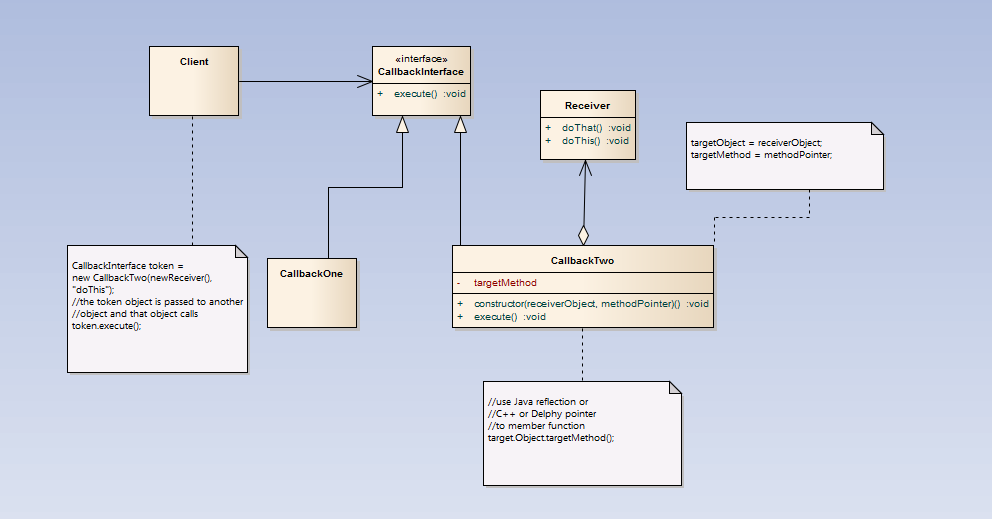
\includegraphics[scale=0.60]{img/pics/command.PNG}
\caption{ \protect \cite{Shvets}}
\label{fig:ref_command}
\end{figure}
\subsubsection{Intent}
\begin{itemize} 
\item Encapsulate a request as an object, thereby letting you parameterize clients with different requests, queue or log requests, and support undoable operations
\item Promote "invocation of a method on an object" to full object status
\item An object-oriented callback
\end{itemize} 
\citep{Shvets}

\subsubsection{Description}
“Command decouples the object that invokes the operation from the one that knows how to perform it. To achieve this separation, the designer creates an abstract base class that maps a receiver (an object) with an action (a pointer to a member function). The base class contains an execute method that simply calls the action on the receiver. All clients of Command objects treat each object as a "black box" by simply invoking the object's virtual execute method whenever the client requires the object's "service". \vfill A Command class holds some subset of the following: an object, a method to be applied to the object, and the arguments to be passed when the method is applied. The Command's "execute" method then causes the pieces to come together.  Sequences of Command objects can be assembled into composite (or macro) commands.”\citep{Shvets}


\subsubsection{Practical usage in game development}
One possible usage for the command pattern in game development is the way how user input is handled. A simple and fast implementation to handle the user input is to hardcode certain functions or actions to fixed buttons. This works as long as there is no need to configure how the buttons are mapped. Otherwise the pattern provides a nice solution to encapsulate the available buttons from their supposed function, by simple mapping the buttons to a command object. In this case, the button calls the execute() function of the command base class and doesn't know or care who the receiver is.

Handling actions within the game with commands opens up the option for the AI to use this too. Instead of hardwiring the AI to the actors, the system could simply send out commands to control an actor.
“The decoupling here between the AI that selects commands and the actor code that performs them gives us a lot of flexibility. We can use different AI modules for different actors. Or we can mix and match AI for different kinds of behavior.”\citep{nystrom2014game}
 
Another useful and common application for the command pattern is the implementation of undo and redo. By storing commands in a list and extending the command object with a undo() function it is easy to implement this functionality. 

\subsection{Flyweight Pattern}
The Flyweight pattern is one of the structural design patterns. It provides a solution for “designing objects down to the lowest levels of system "granularity"[…]” \citep{Shvets}
\begin{figure}[!hbp]
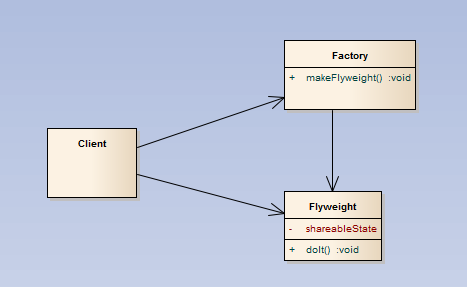
\includegraphics[scale=0.70]{img/pics/flyweight.PNG}
\caption{ \protect \cite{Shvets}}
\label{fig:ref_flyweight}
\end{figure}
\subsubsection{Intent}
\begin{itemize} 
\item Use sharing to support large numbers of fine-grained objects efficiently
\end{itemize} 
\citep{Shvets}
\subsubsection{Description}
“The Flyweight pattern describes how to share objects to allow their use at fine granularities without prohibitive cost. Each "flyweight" object is divided into two pieces: the state-dependent (extrinsic) part, and the state-independent (intrinsic) part. Intrinsic state is stored (shared) in the Flyweight object. Extrinsic state is stored or computed by client objects, and passed to the Flyweight when its operations are invoked.”\citep{Shvets}
“Flyweights are stored in a Factory's repository. The client restrains herself from creating Flyweights directly, and requests them from the Factory. Each Flyweight cannot stand on its own. Any attributes that would make sharing impossible must be supplied by the client whenever a request is made of the Flyweight. If the context lends itself to "economy of scale" (i.e. the client can easily compute or look-up the necessary attributes), then the Flyweight pattern offers appropriate leverage.” \citep{Shvets}
\subsubsection{Practical usage in game development}
A case where this pattern can be of use is, when a large amount of objects that use the same intrinsic values needs to be displayed. 
E.g. render a large forest. By gathering the intrinsic values in one spot, it is possible to pass this information to the GPU once and use it to render all similar objects in the scene, instead of passing it multiple times. 

\subsection{Observer Pattern}
Also a behavior pattern and it allows components to notify other components without knowing which components are affected or how many there are. 

\begin{figure}[!hbp]
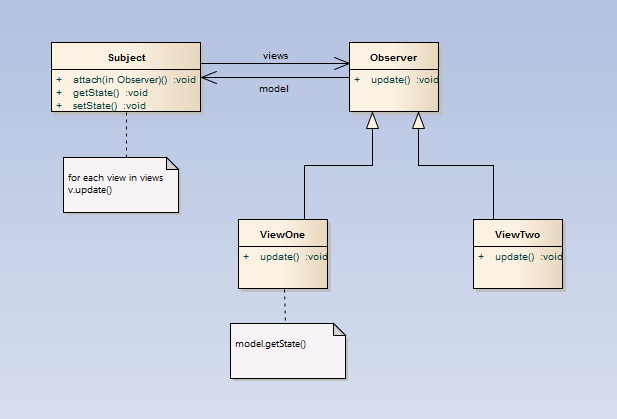
\includegraphics[width=\textwidth, height=8cm]{img/pics/observer.PNG}
\caption{ \protect \cite{Shvets}}
\label{fig:ref_observer}
\end{figure}
\subsubsection{Intent}
\begin{itemize} 
\item Define a one-to-many dependency between objects so that when one object changes state, all its dependents are notified and updated automatically.
\item Encapsulate the core (or common or engine) components in a Subject abstraction, and the variable (or optional or user interface) components in an Observer hierarchy.
\item The "View" part of Model-View-Controller.
\end{itemize} 
\citep{Shvets}
\subsubsection{Description}
“Observers register themselves with the Subject as they are created. Whenever the Subject changes, it broadcasts to all registered Observers that it has changed, and each Observer queries the Subject for that subset of the Subject's state that it is responsible for monitoring. 
The protocol described above specifies a "pull" interaction model. Instead of the Subject "pushing" what has changed to all Observers, each Observer is responsible for "pulling"
\vspace{8cm} \vfill its particular "window of interest" from the Subject. The "push" model compromises reuse, while the "pull" model is less efficient. “\citep{Shvets}

\subsubsection{Practical usage in game development}
One way to use the observer pattern in a game is to implement an achievement system with it.
Achievements can vary wildly in their complexity to unlock them, from simply completing a level to carrying out a series of specific task controlled by different parts of the system. For example, instead of writing checks for achievements directly into the physics code, we extend this part with the subject interface and turn it into a subject. Now the physics code only has to send a notification if something happened that might be of interest for the achievement system. 




\subsection{Decorator/Component Pattern}
A structual pattern which allows to add and remove functionality to an object.

\begin{figure}[!hbp]
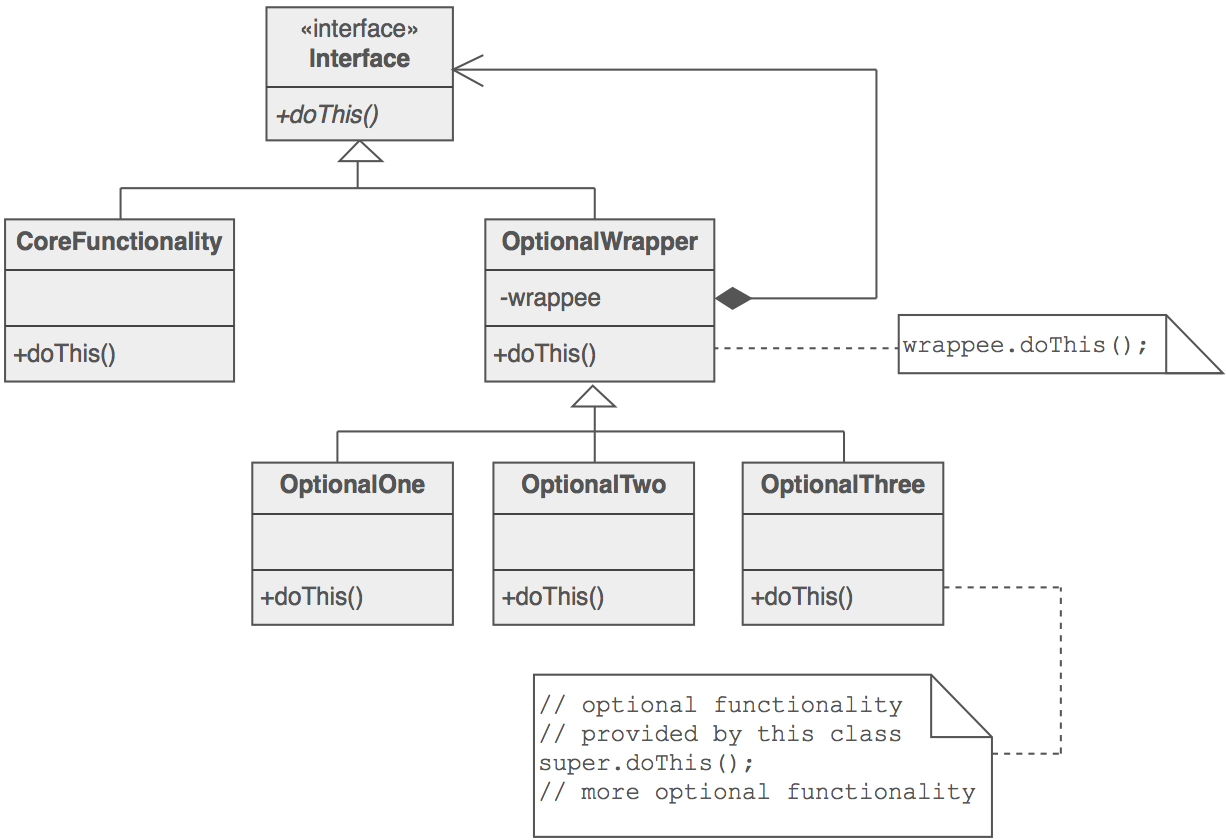
\includegraphics[width=\textwidth, height=8cm]{img/pics/decorator.PNG}
\caption{ \protect \cite{Shvets}}
\label{fig:ref_decorator}
\end{figure}
\subsubsection{Intent}
\begin{itemize} 
\item You have a class that touches multiple domains which you want to keep decoupled from each other.
\item A class is getting massive and hard to work with.
\item You want to be able to define a variety of objects that share different capabilities, but using inheritance doesn’t let you pick the parts you want to reuse precisely enough.
\item Attach additional responsibilities to an object dynamically. Decorators provide a flexible alternative to subclassing for extending functionality.
\end{itemize} 
\citep{Shvets}
\citep{nystrom2014game}

\subsubsection{Description}
The Decorator or Component pattern encapsulates different domains and responsibilities which can be attached or removed dynamically. The concrete object with the desired functionality is simple a container, holding the components. By adding and removing components from the holding container, the behavior and functionality of an object can be altered. It allows building different objects through its flexibility to combine components in an arbitrary manner. Since the actual behavior for the created object is inside the components and is accessed through pointers, the added level of indirection could result in a poorer performance.  

\subsubsection{Practical usage in game development}
A very good opportunity to use this pattern while developing a game is to use it for the backbone functionalities of a game. Physics, graphics, input reading, sound, collision detection, rendering etc. One or more of those parts are probably used by every game object inside a game. To avoid coupling and rewriting the same code parts over and over again, the component pattern is a good solution to this problem. An example of this pattern would be the Unity3D  GameObject and its components. In this engine, all the major parts an object might need to use are separated into their own component which can be simply attached to the container to add its functionality. 




\vfill

\pagebreak
\section{Evaluation of UML Tools}
In this section, I will give you a little overview over some UML tools, I tested. 
\subsection{Enterprise Architect}
The EA is the tool I got the most experience with. If you are just searching for anything to display your UML diagrams, take this one. It is relatively easy to learn and provides anything you need for all types of UML visualization. 
\begin{table}[htbp]
\centering
\begin{tabular}{c|c}
\hline \hline 
Criteria & Result \\ \hline \hline
Name & Enterprise Architect \\ \hline
Version & 10.0.1010 \\ \hline
Vendor & Sparx Systems \\ \hline
License & Ultimate \\ \hline
Model Import/Export & XMI, CSV \\ \hline
Diagram Export & PDF \\ \hline
class diagram & yes \\ \hline
use-case diagram & yes \\ \hline
activity diagram & yes \\ \hline
state diagram & yes \\ \hline
component diagram & yes \\ \hline
requirements diagram & yes \\ \hline
Language & english \\ \hline
OS & Win7/8/10 \\ \hline \hline
\end{tabular}
\caption{Test: Enterprise Architect}
\label{tab:ea}
\end{table}
With the EA it is really easy to create UML diagrams in very short time. If you are more experienced with modelling, you can use it for model-driven source code generation as well. It works out for Java and C\#. Further you can reuse once created classes in multiple diagrams. The project browser allows you to link classes several times and you can follow these links back to the origin. Also useful is the integrated UML compliance guard. If you for example try to connect two use-cases with an inheritance it wont let you do that. So it is also a good support for less experienced UML designers.
\pagebreak
\subsection{Astah}
 Astah is a very potent UML tool, with lots of available diagrams, export formats and customizations in form of plug-ins. Unfortunately it is not free, except for students. 
\begin{table}[htbp]
\centering
\begin{tabular}{c|c}
\hline \hline 
Criteria & Result \\ \hline \hline
Name & Astah Professional \\ \hline
Version & 7.0.0/846701 \\ \hline
Vendor & Astah \\ \hline
License & Trial \\ \hline
Model Import/Export & XMI \\ \hline
Diagram Export & Image, XML, CSV, HTML \\ \hline
class diagram & yes \\ \hline
use-case diagram & yes \\ \hline
activity diagram & yes \\ \hline
state diagram & yes \\ \hline
component diagram & yes \\ \hline
requirements diagram & yes \\ \hline
Language & english, japanese  \\ \hline
OS & Win7/8/10, Linux, MAC OS \\ \hline \hline
\end{tabular}
\caption{Test: Astah Professional}
\label{tab:ea}
\end{table}
Astah is a fully fledged UML Tool. It supports the common UML diagrams and a lot of export types. Importing works via the XML format but it can export various image types, HTML, CSV, RTF and can also export to Java, C\# and C++.  Furthermore Astah can natively convert java files into diagrams. The vendor offers free plug-ins to further customize the application.  For the diagram creation from code files, the vendor already offers the plug-ins for C\# and C++.The User interface is simple and well structured, but it needs some time to really get used to it.
\pagebreak
\pagebreak
\section{Model Driven Development}

\begin{quote}
''models are used for designing systems, understanding them better, specifying required functionality, and creating documentation. Code is then written to implement the designs.''\citep{model-stahl-2006}
\end{quote}

The application of models to software development is a well-known approach and has become even more popular with the introduction of the Unified Modeling Language (UML). In Model-Driven Software Development (MDSD or MDD) an entirely different approach is adopted with respect to the usage of models. MDSD is considered as the natural continuation of the current programming languages and software development methods. In MDSD models do not constitute documentation but are considered equal to code. MDSD aims to utilize domain-specific languages to create models that express application structure and behavior in a more efficient way. The models are then (semi)automatically transformed into executable code by model transformations.

MDD can be defined as a software development methodology with following characteristics:
\begin{enumerate}
\item MDD focuses on the models rather than the code, and the
models are the major artifacts of the software development.
\item Models in MDD are formal thus can be transformed into the
software automatically, or the models are executable.
\item Models are created with a modeling language at a higher abstraction level than the programming language.
\end{enumerate}

Models in MDD can be created with either General Purpose Languages (GPLs), or Domain-Specific Languages (DSLs). UML is the most popular modeling GPL standardized by Object Management Group, which was developed to be able to model all kinds of application domains.
\fref{fig:mdd-concept} shows the concepts of MDD, and their relationships:

\begin{figure}[!htbp]
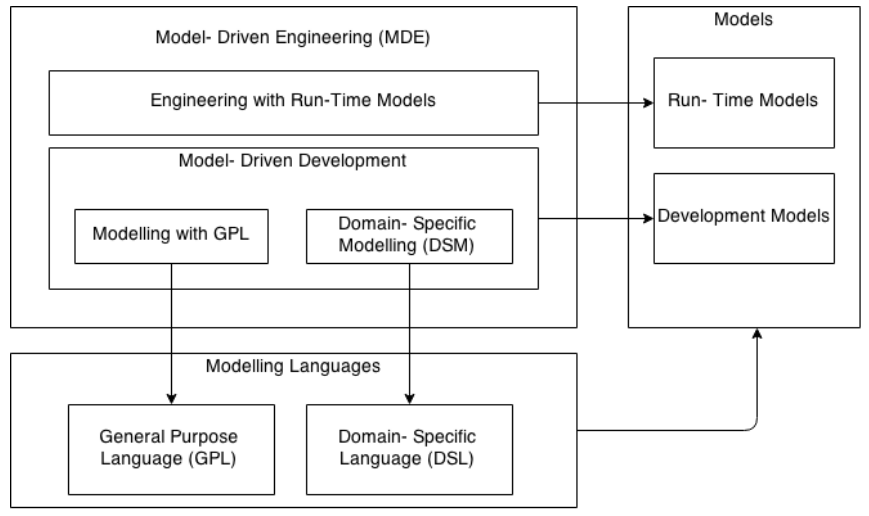
\includegraphics[width=0.5\textwidth]{img/MDD-concept.PNG}
\caption{ MDD concepts and their relationships }
\label{fig:mdd-concept}
\end{figure}

A typical example is the level model created with the level editor, which provides a visual environment for game world modeling. However, the game elements that engine tools can model are restricted to a narrow scope of game software, which are mainly assets like level data and presentation data (\fref{fig:lang-concept}). A lot more elements such as AI, control, rules still have to be handcoded, either with a native language or with a scripting language. Some state-of-art game engines do provided visual modeling tools for creating script code, for example, Unreal Kismet, but these tools are not taking full advantages of MDD, such as use of meta-models and language workbenches, which makes it difficult to be adapted to a new game domain \citep{model-zhu-2014}.

An essential value of MDD is the raised abstraction level, which allows specifying solution with problem domain concepts. To be successful in practice, MDD approaches must find the balance among the abstraction level, the complexity of the language, and the broadness of the domain \citep{model-stahl-2006}.

\begin{figure}[!htbp]
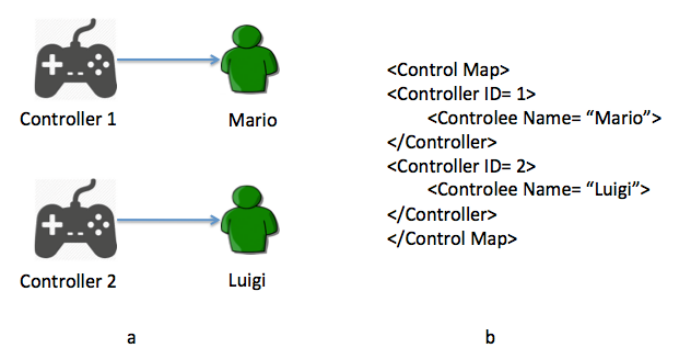
\includegraphics[width=0.5\textwidth]{img/Language-concept.PNG}
\caption{ Graphical Syntax V.S. Textual Syntax }
\label{fig:lang-concept}
\end{figure}

\pagebreak
\subsection{The Goals of MDSD}

\begin{enumerate}
\item Runnable code can be generated from formal models using one or more transformation steps.
\item The use of automated transformations and formally-defined modeling languages lets you enhance software quality.
\item Better maintainability of software systems through redundancy avoidance and manageability of technological changes.
\item Architectures, modeling languages and transformations can be used in the sense of a software production line for the manufacture of diverse software systems. This leads to a higher level of reusability and makes expert knowledge widely available in software form.
\item Another significant potential is the improved manageability of complexity through abstraction.
\item MDSD offers a productive environment in the technology, engineering, and management fields through its use of process building blocks and best practices.
\end{enumerate}

\vfill\break
\subsection{Basic Concept}

Domain-related specifications are defined in Platform-Independent Models (PIMs). A formal modeling language is used that is specific to the concepts of the domain to be modeled. In most cases, one would use UML that has been adapted via profiles to the respective domain, not least because of its tool support. These domain-specific descriptions are completely independent of the later implementation on the target platform. \fref{fig:MDA-basic} illustrates this basic principle.

Via model transformation, usually automated with tools, Platform-Specific Models (PSMs) are created from the Platform-Independent Models. These Platform-Specific Models contain the target platform’s specific concepts. The implementation for a concrete target platform is then generated with another tool-supported transformation based on one or more PSMs.

\begin{strip}
    \centering\noindent
    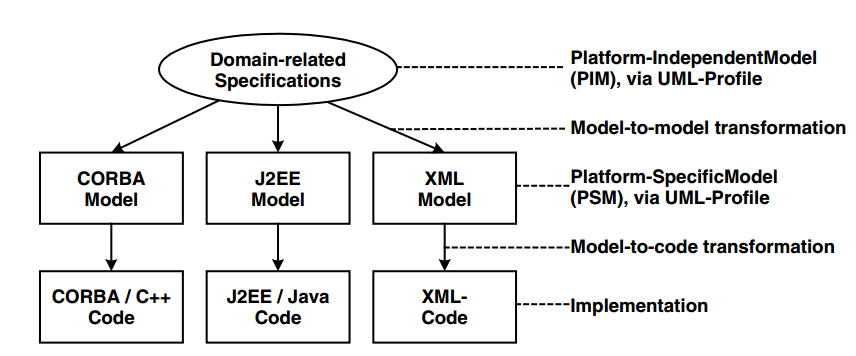
\includegraphics[scale = 0.7]{img/MDA-basic.PNG}
    \captionof{figure}{ Basic concept of MDA Transformation}
    \label{fig:MDA-basic}
\end{strip}


%how to implement a table...

%\begin{table}[htbp]
%\centering
%\begin{tabular}{c|c}
%Bereich & f [Hz] \\ \hline \hline
%Anfang & 194 \\ \hline
%Mitte & 229 \\ \hline
%Ende & 220
%\end{tabular}
%\caption{Ergebnis Median Frequenzen}
%\label{tab:medfrequ}
%\end{table}

% this is a columnbreak
%\vfill\break

%this is how to add a picture
%\begin{figure}[!hbp]
%
\includegraphics[scale = 0.5]{img/test3.png}
%\caption{ caption \protect with citation \cite{smeets_throwing_2002}}
%\label{fig:test1}
%\end{figure}

%in \fref{fig:test1} - this was a reference to a figure using the label!


%-- figure over both columns

%\begin{figure*}[!hbp]
%
\includegraphics[scale = 0.5]{img/test3.png}
%\caption{ caption \protect with citation %\cite{smeets_throwing_2002}}
%\label{fig:test1}
%\end{figure*}

% Bibliography



% Option 1: Bibliography generation with BibTeX:
% Add all refernces to the *.bib file (here Literatur.bib). Then run LaTeX, BibTeX, and again twice LaTeX.
% Use \cite{kop05} within the text for a citation.
% - GEMRAN ----------
%\bibliographystyle{apalike-url-de} %ermöglicht longnamesfirst Option. Bei erster Erwähnung werden alle Autoren gennannt in der Folge et al. verwenden wir aber nicht
% - END GERMAN-------
%% -ENGLISH---------

%\pagebreak
%\bibliographystyle{apalike-url}
%%% -END ENGLISH------
%\bibliography{Bibliography-SoftwareArchitecture}
% Option 2: Bibliography generation without BibTeX:
%\begin{thebibliography}{99}
%\bibitem[kop05]{kop05}
%H.~Kopka, {\em LaTeX, Band 1: Einf"uhrung}, Pearson Studium, M"unchen, 3.~Auflage, 2005.
%\bibitem[knu98]{knu98}
%F.~Mittelbach, M.~Goossens, J.~Braams, D.~Carlisle, and Ch. Rowley, {\em The LaTeX Companion}, 
%Addison-Wesley, 2nd edition, 2004.
%\end{thebibliography}

%\end{document}